\documentclass[a4paper,twoside]{article}
\usepackage{graphicx}
\usepackage{epsfig}
\usepackage{subcaption}
\usepackage{calc}
\usepackage{amssymb}
\usepackage{amstext}
\usepackage{amsmath}
\usepackage{amsthm}
\usepackage{multicol}
\usepackage{pslatex}
\usepackage{apalike}
\usepackage[bottom]{footmisc}
\usepackage{SCITEPRESS}     % Please add other packages that you may need BEFORE the SCITEPRESS.sty package.

%Path relative to the .tex file containing the \includegraphics command
\graphicspath{ {images/} }

% ============ Begin Document =========================
\begin{document}

\title{An Ontology-based Knowledge Management Model on Information Governance}

\author{\authorname{Cataldo Mega\sup{1}\orcidAuthor{/0000-0002-2816-2699}}
\affiliation{\sup{1}Parallel and Distributed Systems Department of Information Systems University of Stuttgart}
\email{cataldo.mega@ipvs.uni-stuttgart.de}
}
%
\keywords{Enterprise Information Management, Information Governance, Ontology, Knowledge Graph, Cloud-Services.}
% ============ Abstrcat ================================================ 
%\abstract{
Information is a strategic asset to enterprises and subject to Information Governance (IG) as mandated by corporate and regulatory compliance. Overall governance goals are the management and control of business relevant data such to minimize legal risks and reduce operational cost. Recent surveys show that around 40\% of companies have insufficient IG practices in place and are exposed to higher compliance risks. Where there exists an IG Strategy, its implementation is typically homegrown, difficult to integrate and error prone. Our investigation shows that a major impediment to implementation and interoperability is the lack of a common language. One that defines what information governance consists of in technical and operational terms. In addition, the many existing frameworks in this domain make the exploitation of the available knowledge and definition of standardized IG specific services very difficult, often leading to costly one-off implementations. A solution to this problem is the availability of a common and unambiguous domain vocabulary as a pre-requisite to a commonly accepted ontology on information governance. This paper suggests an ontology-based framework (IGONTO) that supports the creation of a knowledge store that facilitates access of domain knowledge through semantic search.
}

\abstract{Information is a strategic asset to enterprises and subject to Information Governance (IG) as mandated by corporate and regulatory compliance. Overall governance goals are the management and control of business relevant data such to minimize legal risks and reduce operational cost. Recent surveys show that around 40\% of companies have insufficient IG practices in place and are exposed to higher compliance risks. Where there exists an IG Strategy, its implementation is typically homegrown, difficult to integrate and error prone. Our investigation shows that a major impediment to implementation and interoperability is the lack of a common language. One that defines what information governance consists of in technical and operational terms. In addition, the many existing frameworks in this domain make the exploitation of the available knowledge and definition of standardized IG specific services very difficult, often leading to costly one-off implementations. A solution to this problem is the availability of a common and unambiguous domain vocabulary as a pre-requisite to a commonly accepted ontology on information governance. This paper suggests an ontology-based framework (IGONTO) that supports the creation of a knowledge store that facilitates access of domain knowledge through semantic search.}
\onecolumn \maketitle \normalsize \setcounter{footnote}{0} \vfill
%
% ============ Chap1 Introduction =========================
%
%\section{\uppercase{introduction}}
\label{sec:INTRODUCTION}
Our work is premised on the basis that domain knowledge, expertise and technology on information governance solutions exist in abundance but scattered around and difficult to get hold on. In order to aid companies to find the blueprint of an IG solution that suites their needs the existing knowledge must be collected, synthesized, and offered as a service, accessible to humans and machines in an easy and cost-effective way. We believe this is best done through the use of an ontology-based model on information governance. Our suggestion is to create an information governance graph based on an ontology constructed with a rich semantic model. We envision a graph store containing generalized information of governance concepts, components modelled from functional, non-functional and operational requirements together with a list of design artefacts that expose key IG capabilities and functions. Figure 1 outlines this approach showing the processing pipeline. Starting from left to right you see: Step 1 knowledge acquisition phase, where, vocabularies terms, guidelines, standards, and best practices are acquired from the IG domain. Step 2 processing phase, the information is processed in to a taxonomy of related concepts, associated rule sets and their descriptions. Step 3 access phase, this is where we create the semantic schema and load instance data (individuals) in to the knowledge graph.  Step 4 delivery phase, at this point users are able to retrieve design models and service templates as constituent parts of an IG solution blueprint and build plans. The result is IGONTO a framework consisting of a harmonized information governance vocabulary, a semantic schema (IGO) and a knowledge graph (IGG). Complementing the framework, we also created a repository of design artefacts in aid of the development of IG solutions. The aim is to provides a way for interested parties to use the framework as a knowledge system for generating state-of-the-art design models and building blocks such for being able to compose an envisioned IG solution. 
The remainder of this paper details our approach and is structured as follows: Section 1.1 introduces briefly some of the key aspects of the governance domain but focusing on information governance. Section 1.2 describes the business problem. Section 1.3 motivates a solution with a concrete use case scenario. Section 2 discusses the governance domain analysis we conducted. Section 2.1 lists our contributions. Section 3 uses the results of the analysis to introduce the taxonomy and the IG knowledge models which we created. Section 4 presents related work. Section 5 has concluding remarks and an outlook.

\begin{figure*}[!hbtp]
  \centering
%   \includegraphics[width=\textwidth]{images/iceis-fig01.png}
   \includegraphics[width=\textwidth]{images/Fig1-Processpipe.png}
%    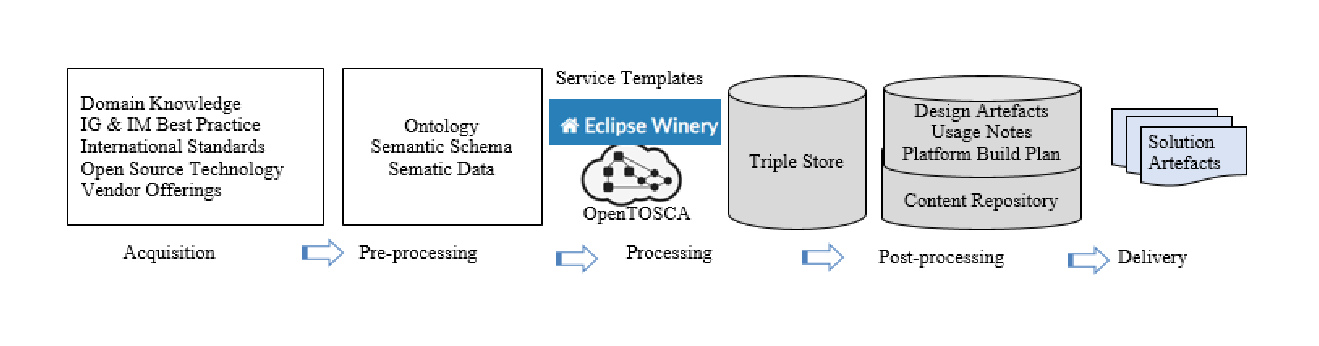
\includegraphics[width=\ScaleIfNeeded]{images/Bild1-2b.pdf}
    \caption{Process pipeline from knowledge acquisition to service implementation.}
  \label{fig:procpipe}
\end{figure*}
%\twocolumn
%\clearpage
\subsection{{Governance Domains}}
Governance at its core is about corporate and regulatory compliance. It is based on trust fueled by continuous IG practice, monitoring its effectiveness and control. This implies responsibilities and commitments realized through processes that ensure proper data access, implement guidelines and legal requirements. As such, corporate governance (CG) in an enterprise ensures that valuable information adhere with proper quality standards related to data authenticity, integrity and reliability in compliance with regulations. Thus enterprises are governed by a framework of principles, values, policies and processes intended to help organizational units to move towards shared corporate compliance goals. 
The principal design criteria of governance have a focus on enabling information quality strategies and to classify process capabilities against an Information Governance Maturity Model (Pierce, 2007). This means, at its core governance models cover three major responsibility domains: Corporate Governance (CG), Information Governance (IG) and IT Governance (ITG) outlined in Figure 2. Each domain addresses different governance areas using frameworks suitable for one or the other, emphasizing more the organizational or implementation aspects. 
The left-hand side of Figure 2 shows Information Governance and its relations to the categories of Information Management, Content Management, Records Management and Asset Management. These categories represent the context in which data is processed under the scrutiny of information governance lifecycles. The latter being workflows that perform activities to apply compliance policies and enforce rules on how to handle corporate data and information. Similarly, IT Governance, as shown on the right-hand side, relates to IT-Operations rules applied to infrastructure, processes. Thus, in the end governance means to enforce corporate compliance goals ensuring accountability and transparency such to minimize possible risks. 
The focus of the remainder of this paper is on information governance (IG) with occasional references to the other domains, where required.

%\vfill
\subsection{Problem Description}
From experience we learned that the success of information governance and regulatory compliance in companies depends on a common understanding conveyed through an unambiguous language. Such a language is an important pre-requisite to design, implementation and deployment of the required data governance services and their controls. In addition, an information governance strategy depends also on the type of data processed and the business context they belong to. For organizations this implies a responsibility to implement information governance practices that enforce proper data usage in their specific production environment throughout the entire information lifecycle. 
The problem though is that even after knowing ‘what is’ required, many companies face challenges with the architecture design of their individual IG solution because of the many technology and product options available on the market. 
These circumstances translate into a lengthy and formal process of announcing new information governance projects through a Request for Proposal (RFP) where in response, qualified contractors submit bids to undertake the project. Typically, the RFP document contains detailed information about the project, requirements, and evaluation criteria. 
The good news is that typical information governance solutions follow on an architecture blueprint that is composed of well-known software design patterns, available domain knowledge and experience. Luckily enough, software instances of IG building blocks are available in a variety of IG product offerings from open source and different vendors. Therefore, our conclusion is that by exploiting the available knowledge it is possible to generate the required information on components and design artefacts and allowing companies to compose IG solutions instead of custom developing new ones. Which is the goal of our approach outlined in Figure 1. This motivate the use of ontologies and knowledge graphs to store domain knowledge and to make it available through semantic search. The expected benefit is that on a global and open information market this knowledge facilitates the sharing of data and services. We think ontologies can expedite access and retrieval of IG service building blocks where the requirements defined in concept entities are matched by the capabilities of design entities. 
%
\begin{figure}[h]
  \centering
%    \includegraphics[clip, trim=1cm 7cm 0 0 , width=7.5cm]{images/iceis-fig02.png}
    \includegraphics[clip, trim=1cm 7cm 0 0 , width=7.5cm]{images/Fig2-CG.Domains.png}
    \caption{Corporate Governance Domains.}
  \label{fig:igdomains}
\end{figure}
\\ Figure 2: Corporate governance domains

\subsection{Usage Scenario}
Let us look at a real-world IG use case scenario to better explain our approach. Assume a company having the following business requisites: 
•	Business Data: Personal Identifiable Information (PII), customer contractual data and related contextual information; 
•	Businesses domiciled in: US, EU; 
•	Jurisdictions: US, EU; 
•	Regulations: US Privacy Act, EU GDPR; 
Regulatory compliance with these business requisites translates into the following functional and non-functional requirements:
•	R1: Contractual and legal obligations require to collect and classify person and business data as well as related information from pre-contract and contract activities (the context). 
•	 R2: Data is persisted reliably, after verifying its authenticity and integrity. 
•	R3: Data is stored for as long as required by business, legislations and regulations. 
•	R4: Access to stored data is controlled by security and privacy policies. 
•	R5: Data is deleted or barred from access upon lapse of a storage period prescribed by business or legal instruments. 
Figure 3 outlines the use case scenario in form of a semantic graph which we subdivided into three functional arias: Governance (top), Implementation (middle) and Platform (bottom). Note: Capitalized terms printed in bold represent key domain concepts. 
The upper part outlines the business requisites and reads like this: at corporate level a Company has a business presence in the Countries: EU and US. Their Jurisdictions are regulated by the US Privacy Act (GSA, 2022)and the EU GDPR Regulations (EU, 2018). Thus, this Company by law must instate an IG-Program consisting of a number of governance principles that address at the least: Security, Privacy, Integrity and Authenticity concerns in order to reach a maturity level Essential (L3 of L5).
%
\begin{figure*}[!hbtp]
  \centering
%   \includegraphics[width=\textwidth]{images/iceis-fig03.png}
   \includegraphics[width=\textwidth]{images/Fig3-IG.Scenario.png}
    \caption{Process pipeline from knowledge acquisition to service implementation.}
  \label{fig:igscenario}
\end{figure*}
%
 This means, each category consists of a number of obligations and implementation requirements to be satisfied. These are: 
•	R6: verify Data Authenticity, 
•	R7: ensure Data Integrity and 
•	R8: provide system and Service Reliability. 
From an implementation stand point these requirements translate into the following information governance guidelines:
 •	GL1: “…in order to reach a governance maturity Essential (level 3) an organization must implement a Metadata Definition Process that is an integral part of the implemented Records Management Practice”. See Figure 3.
 In addition, the US Privacy Act mandates that:
 •	GL2: “… Data integrity failures must be monitored, assessed, and mitigated …”.  
The center of Figure 3 lists the concept classes mentioned in the guidelines: Data, Metadata, and Records Management Practice. They all relate to processes that satisfy the associated requirements by means of inferred implementation and platform components. For example: Repository, RDBMS, Content Services as shown on the bottom of  Figure 3 
%
The line of thought at concept level follows this logic: The Metadata Definition Process is responsible for creating necessary governance metadata that describe how data is processed and stored based on applicable corporate and regulatory Policies. 
By following well known domain best practices, implementing such an IG-Program implies the presence of repositories where Data and related Metadata is securely stored. In this context, data is subject to different Lifecycles and controlled by a Records Management System. 
Records Classification processes classify the data in to categories and assign specific policies used to control classification, access, retention and disposition by means of appropriate Rules. 
Corporate repositories typically use Databases, Full Text Indexes and Storage Systems representing IT-Resources that today are best provisioned by Platform Services. 
 In a subsequent refinement step the IG concepts are then mapped on to solution component models and implementation classes where concept links are translated into class relationships. For example, following nodes at the bottom of Figure 3 one gets: 
Repository -> Content Repository-> Content Services -> Alfresco Content Services  •	Repository -> Metadata Repository -> Database Service -> Database ->PostgreSQL. 
With this approach, it is possible to identify the required components and design an IG solution following the architecture blueprint shown in Figure 4. From left to right, Figure 4 outlines how data is processed. Starting from the data sources where data is pre-processed and classified. Qualified data is then collected and loaded in an enterprise information systems (EIS) and put under control of information lifecycles. Governance lifecycle processes create required governance metadata before both data and metadata are persisted in an enterprise repository typically a Content Management (ECM) system. Post-processing, shown on the right side of Figure 4, is performed by Enterprise Records, Case Management, eDiscovery and Content Analytics components.  These services produce required governance information such to satisfy audit trails, statistics and reporting needs. 
At the high level Figure 3 represents the concept and  Figure 4  the implementation domain describing the mapping between concept, classes and components. The gist of what this use case is trying to convey is that with the given business requisites and based on the defined semantic model, it is possible to generate concept artefacts having the capabilities and characteristics for satisfying the implied functional, non-functional and operational requirements with the aid of a knowledge store. 
In summary we observe that a successful IG-Program implementation depends directly on an efficient enterprise information system where governance is achieved through adjustments of the information management practice with ongoing monitoring, assessment and reporting.
\section{\uppercase{introduction}}
\label{sec:INTRODUCTION}
Our work is premised on the basis that domain knowledge, expertise and technology on information governance solutions exist in abundance but scattered around and difficult to get hold on. In order to aid companies to find the blueprint of an IG solution that suites their needs the existing knowledge must be collected, synthesized, and offered as a service, accessible to humans and machines in an easy and cost-effective way. We believe this is best done through the use of an ontology-based model on information governance. Our suggestion is to create an information governance graph based on an ontology constructed with a rich semantic model. We envision a graph store containing generalized information of governance concepts, components modelled from functional, non-functional and operational requirements together with a list of design artefacts that expose key IG capabilities and functions. Figure 1 outlines this approach showing the processing pipeline. Starting from left to right you see: Step 1 knowledge acquisition phase, where, vocabularies terms, guidelines, standards, and best practices are acquired from the IG domain. Step 2 processing phase, the information is processed in to a taxonomy of related concepts, associated rule sets and their descriptions. Step 3 access phase, this is where we create the semantic schema and load instance data (individuals) in to the knowledge graph.  Step 4 delivery phase, at this point users are able to retrieve design models and service templates as constituent parts of an IG solution blueprint and build plans. The result is IGONTO a framework consisting of a harmonized information governance vocabulary, a semantic schema (IGO) and a knowledge graph (IGG). Complementing the framework, we also created a repository of design artefacts in aid of the development of IG solutions. The aim is to provides a way for interested parties to use the framework as a knowledge system for generating state-of-the-art design models and building blocks such for being able to compose an envisioned IG solution. 
The remainder of this paper details our approach and is structured as follows: Section 1.1 introduces briefly some of the key aspects of the governance domain but focusing on information governance. Section 1.2 describes the business problem. Section 1.3 motivates a solution with a concrete use case scenario. Section 2 discusses the governance domain analysis we conducted. Section 2.1 lists our contributions. Section 3 uses the results of the analysis to introduce the taxonomy and the IG knowledge models which we created. Section 4 presents related work. Section 5 has concluding remarks and an outlook.

\begin{figure*}[!hbtp]
  \centering
%   \includegraphics[width=\textwidth]{images/iceis-fig01.png}
   \includegraphics[width=\textwidth]{images/Fig1-Processpipe.png}
%    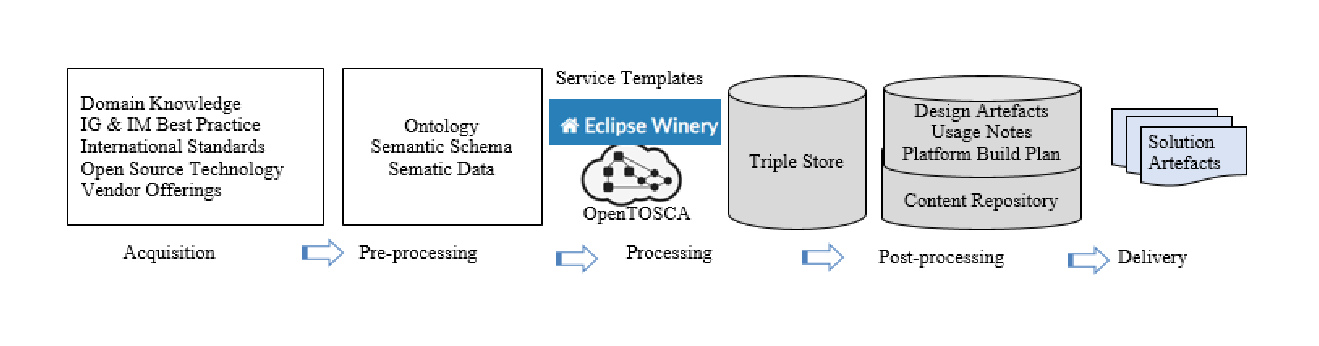
\includegraphics[width=\ScaleIfNeeded]{images/Bild1-2b.pdf}
    \caption{Process pipeline from knowledge acquisition to service implementation.}
  \label{fig:procpipe}
\end{figure*}
%\twocolumn
%\clearpage
% =====================================================================
\subsection{{Governance Domains}}
Governance at its core is about corporate and regulatory compliance. It is based on trust fueled by continuous IG practice, monitoring its effectiveness and control. This implies responsibilities and commitments realized through processes that ensure proper data access, implement guidelines and legal requirements. As such, corporate governance (CG) in an enterprise ensures that valuable information adhere with proper quality standards related to data authenticity, integrity and reliability in compliance with regulations. Thus enterprises are governed by a framework of principles, values, policies and processes intended to help organizational units to move towards shared corporate compliance goals. 
The principal design criteria of governance have a focus on enabling information quality strategies and to classify process capabilities against an Information Governance Maturity Model (Pierce, 2007). This means, at its core governance models cover three major responsibility domains: Corporate Governance (CG), Information Governance (IG) and IT Governance (ITG) outlined in Figure 2. Each domain addresses different governance areas using frameworks suitable for one or the other, emphasizing more the organizational or implementation aspects. 
The left-hand side of Figure 2 shows Information Governance and its relations to the categories of Information Management, Content Management, Records Management and Asset Management. These categories represent the context in which data is processed under the scrutiny of information governance lifecycles. The latter being workflows that perform activities to apply compliance policies and enforce rules on how to handle corporate data and information. Similarly, IT Governance, as shown on the right-hand side, relates to IT-Operations rules applied to infrastructure, processes. Thus, in the end governance means to enforce corporate compliance goals ensuring accountability and transparency such to minimize possible risks. 
The focus of the remainder of this paper is on information governance (IG) with occasional references to the other domains, where required.
%\vfill
% =====================================================================
\subsection{Problem Description}
From experience we learned that the success of information governance and regulatory compliance in companies depends on a common understanding conveyed through an unambiguous language. Such a language is an important pre-requisite to design, implementation and deployment of the required data governance services and their controls. In addition, an information governance strategy depends also on the type of data processed and the business context they belong to. For organizations this implies a responsibility to implement information governance practices that enforce proper data usage in their specific production environment throughout the entire information lifecycle. 
The problem though is that even after knowing ‘what is’ required, many companies face challenges with the architecture design of their individual IG solution because of the many technology and product options available on the market. 
These circumstances translate into a lengthy and formal process of announcing new information governance projects through a Request for Proposal (RFP) where in response, qualified contractors submit bids to undertake the project. Typically, the RFP document contains detailed information about the project, requirements, and evaluation criteria. 
The good news is that typical information governance solutions follow on an architecture blueprint that is composed of well-known software design patterns, available domain knowledge and experience. Luckily enough, software instances of IG building blocks are available in a variety of IG product offerings from open source and different vendors. Therefore, our conclusion is that by exploiting the available knowledge it is possible to generate the required information on components and design artefacts and allowing companies to compose IG solutions instead of custom developing new ones. Which is the goal of our approach outlined in Figure 1. This motivate the use of ontologies and knowledge graphs to store domain knowledge and to make it available through semantic search. The expected benefit is that on a global and open information market this knowledge facilitates the sharing of data and services. We think ontologies can expedite access and retrieval of IG service building blocks where the requirements defined in concept entities are matched by the capabilities of design entities. 
%
\begin{figure}[ht]
  \centering
%    \includegraphics[clip, trim=1cm 7cm 0 0 , width=7.5cm]{images/iceis-fig02.png}
    \includegraphics[clip, trim=1cm 7cm 0 0 , width=7.5cm]{images/Fig2-CG.Domains.png}
    \caption{Corporate Governance Domains.}
  \label{fig:g-domains}
\end{figure}
\\ Figure 2: Corporate governance domains
% ======================================================================
\subsection{Usage Scenario}
Let us look at a real-world IG use case scenario to better explain our approach. Assume a company having the following business requisites: 
•	Business Data: Personal Identifiable Information (PII), customer contractual data and related contextual information; 
•	Businesses domiciled in: US, EU; 
•	Jurisdictions: US, EU; 
•	Regulations: US Privacy Act, EU GDPR; 
Regulatory compliance with these business requisites translates into the following functional and non-functional requirements:
•	R1: Contractual and legal obligations require to collect and classify person and business data as well as related information from pre-contract and contract activities (the context). 
•	 R2: Data is persisted reliably, after verifying its authenticity and integrity. 
•	R3: Data is stored for as long as required by business, legislations and regulations. 
•	R4: Access to stored data is controlled by security and privacy policies. 
•	R5: Data is deleted or barred from access upon lapse of a storage period prescribed by business or legal instruments. 
Figure 3 outlines the use case scenario in form of a semantic graph which we subdivided into three functional arias: Governance (top), Implementation (middle) and Platform (bottom). Note: Capitalized terms printed in bold represent key domain concepts. 
The upper part outlines the business requisites and reads like this: at corporate level a Company has a business presence in the Countries: EU and US. Their Jurisdictions are regulated by the US Privacy Act (GSA, 2022)and the EU GDPR Regulations (EU, 2018). Thus, this Company by law must instate an IG-Program consisting of a number of governance principles that address at the least: Security, Privacy, Integrity and Authenticity concerns in order to reach a maturity level Essential (L3 of L5).
%
\begin{figure*}[!hbtp]
  \centering
%   \includegraphics[width=\textwidth]{images/iceis-fig03.png}
   \includegraphics[width=\textwidth]{images/Fig3-IG.Scenario.png}
    \caption{IG scenarios and use cases.}
  \label{fig:scenarios}
\end{figure*}
%
 This means, each category consists of a number of obligations and implementation requirements to be satisfied. These are: 
•	R6: verify Data Authenticity, 
•	R7: ensure Data Integrity and 
•	R8: provide system and Service Reliability. 
From an implementation stand point these requirements translate into the following information governance guidelines:
 •	GL1: “…in order to reach a governance maturity Essential (level 3) an organization must implement a Metadata Definition Process that is an integral part of the implemented Records Management Practice”. See Figure 3.
 In addition, the US Privacy Act mandates that:
 •	GL2: “… Data integrity failures must be monitored, assessed, and mitigated …”.  
The center of Figure 3 lists the concept classes mentioned in the guidelines: Data, Metadata, and Records Management Practice. They all relate to processes that satisfy the associated requirements by means of inferred implementation and platform components. For example: Repository, RDBMS, Content Services as shown on the bottom of  Figure 3 
%
The line of thought at concept level follows this logic: The Metadata Definition Process is responsible for creating necessary governance metadata that describe how data is processed and stored based on applicable corporate and regulatory Policies. 
By following well known domain best practices, implementing such an IG-Program implies the presence of repositories where Data and related Metadata is securely stored. In this context, data is subject to different Lifecycles and controlled by a Records Management System. 
Records Classification processes classify the data in to categories and assign specific policies used to control classification, access, retention and disposition by means of appropriate Rules. 
Corporate repositories typically use Databases, Full Text Indexes and Storage Systems representing IT-Resources that today are best provisioned by Platform Services. 
 In a subsequent refinement step the IG concepts are then mapped on to solution component models and implementation classes where concept links are translated into class relationships. For example, following nodes at the bottom of Figure 3 one gets: 
Repository -> Content Repository-> Content Services -> Alfresco Content Services  •	Repository -> Metadata Repository -> Database Service -> Database ->PostgreSQL. 
With this approach, it is possible to identify the required components and design an IG solution following the architecture blueprint shown in Figure 4. From left to right, Figure 4 outlines how data is processed. Starting from the data sources where data is pre-processed and classified. Qualified data is then collected and loaded in an enterprise information systems (EIS) and put under control of information lifecycles. Governance lifecycle processes create required governance metadata before both data and metadata are persisted in an enterprise repository typically a Content Management (ECM) system. Post-processing, shown on the right side of Figure 4, is performed by Enterprise Records, Case Management, eDiscovery and Content Analytics components.  These services produce required governance information such to satisfy audit trails, statistics and reporting needs. 
At the high level Figure 3 represents the concept and  Figure 4  the implementation domain describing the mapping between concept, classes and components. The gist of what this use case is trying to convey is that with the given business requisites and based on the defined semantic model, it is possible to generate concept artefacts having the capabilities and characteristics for satisfying the implied functional, non-functional and operational requirements with the aid of a knowledge store. 
In summary we observe that a successful IG-Program implementation depends directly on an efficient enterprise information system where governance is achieved through adjustments of the information management practice with ongoing monitoring, assessment and reporting.
% 
% ============ Chap2 IG DOMAIN ANALYSIS ========================
%\section{IG DOMAIN ANALYSIS}
\label{sec:domainanalysis}
This section briefly introduces the domain sources we evaluated in our effort to identify valuable IG knowledge, concept classes and their meaning. Table 1 shows a representative list of practitioner organizations and public agencies, their frameworks and scope. Common to the taxonomy employed by each framework is a 3-level category structure. Column 2 in Table 1 outlines the overall scope of each governance frameworks and its functional areas. These are: General Governance Principles (IGMM), IG Reference Model (IGRM), Electronic Discovery Reference Model (EDRM), IT Governance Suite, Digital Asset Management, and Data Management Framework.
%table1 
\begin{table}[h]
\caption{IG Frameworks.}
\label{tab:example1} \centering
\scalebox{0.55} {\begin{tabular} {|l|l|}
  \hline
  Organization & Framework\/Scope\\
  \hline
  ARMA & {IGMM - IG Maturity Model – Principles}\\
  \hline
  {CGOC / EDRM} & {IG Reference Model, Electronic Discovery Reference Model}\\
  \hline
  {ISACA	COBIT} & {IT Governance Suite} \\
  \hline
  {DAM}	& {Digital Asset Management} \\
  \hline
  {DAMA} 	& {Data Management Framework} \\
  \hline
  {NARA } &  {(NARA, 2006) National Archives and Records Administration} \\
  \hline 
  {Records Management}  & {Center of Research Libraries} \\
  \hline
 \end{tabular}}
\end{table}
%
The main categories used across the frameworks are: Accountability, Transparency, Integrity, Protection, Compliance, Availability, Retention and Disposition. These categories become principles. They apply for the organizational or functional areas and play an essential role when implementing an IG-Program. See Figure 3. Each principle has a number of context specific capabilities and/or requirements assigned. They represent concept/class attributes or relationship properties. The frameworks also introduced a scalar metric called governance maturity level (GML), with a value range from 0 to 5 (i.e. ad ranging from ad hoc to a fully functional IG-Program implementation). A GML is computed from a specific subset of capabilities and requirements that must be satisfied by context and category. The last row of Table 1 lists (NARA, 2006) and CRL both represent government agencies. They share frameworks with a focus on the records management lifecycles and aspects to manage and operate Records-, Content Management System and Digital Archives. Their guidelines draw requirements from relevant standards like NIST.IR.8286C Staging Cybersecurity Risks for Enterprise Risk Management and Governance Oversight \cite{Quinn2022} and ISO-15489 Information and documentation — Records management \cite{ISO15489}. We evaluated also international ISO standards for the applicable domain as listed in Table 2. 
%table 2
\begin{table}[h]
\caption{Table 2: ISO Standards.}
\label{tab:example1} \centering
 \scalebox{0.55} {\begin{tabular}{|l|l|}
 %\begin{tabular}{|c|>{\raggedleft\arraybackslash}l|}
 \hline
  {Organization} & {Standards}\\
  \hline
  {ISO Standards}	 & {}\\
  \hline
  {ISO-14271} & {Open Archive Information System}\\
  \hline
  {ISO-15489} & {Records Management: Concepts and Principles} \\
  \hline
  {ISO-16363}	& {Audit and certification} \\
  \hline
  {ISO-27000} & {Information Security Management Systems (ISMS) standards} \\
  \hline 
  {-}  & {including Information security} \\
  {-}  & {cybersecurity and privacy protection } \\
  {-}  & {risk management guidelines} \\
  {(ISO-37301, 2021)}  & {Compliance Management systems } \\
  \hline
 \end{tabular}}
\end{table}
%
Table 3 shows 3 privacy regulations in force in the US, EU and DE jurisdictions. We included them as they represent the security and privacy categories. The two major principles information governance these days. 
%
%table 3
\begin{table}[h]
\caption{Table 3: Regulators and Regulations.}
\label{tab:example1} \centering
 \scalebox{0.55} {\begin{tabular}{|l|l|}
 %\begin{tabular}{|c|>{\raggedleft\arraybackslash}l|}
 \hline
  {Regulator} & {Regulations}\\
  \hline
  {US-GSA} & {US Government Services Agency Directives: Privacy Act \cite{USGSA}}\\
  \hline
  {Germany} & {DE Datenschutz-Grundverordnung} \\
  \hline 
 \end{tabular}}
\end{table}
%
Interesting to note: Ensuring compliance with these regulations already employs a complex implementation model. It involves elements of core Enterprise Information Systems (EIS) concepts, like the ones introduced and discussed in the use case scenario. 
In moving from business to implementation concepts we searched for standards related to enterprise information management (EIM) systems and looked at their design models. The 3 Standards of interest are listed in Table 4. These are the 2 OASIS standards: 1) CMIS, the “Content Management Interoperability Services” standard, 2) TOSCA the “Topology and Orchestration of Specification for Cloud Applications” and 3) the “Trustworthy Digital Repositories” specification which was standardized in ISO-14271
%table4 
\begin{table}[h]
\caption{The ECM Blueprint, Design, Deployment and Cloud Orchestration Standards.}
\label{tab:example1} \centering
 \scalebox{0.55} {\begin{tabular}{|l|l|}
 %\begin{tabular}{|c|>{\raggedleft\arraybackslash}l|}
 \hline
  {Organization} & {Standards}\\
  \hline
  {OASIS} & {CMIS Content Management Interoperability Services \cite{CMIS}}\\
  \hline
  {OASIS} & {TOSCA Topology and Orchestration Specification } \\
  {} & { for Cloud Applications \cite{TOSCA}} \\  
  \hline 
  {ISO / NASA} & { Trustworthy Digital Repositories \cite{ISO14721}}\\
  \hline
 \end{tabular}}
\end{table}
%
All three standards are well suited for our approach as they provide the required links between the business/governance and systems design concepts. In order to create a complementary IG graph store (IGG), we collected concept\/class instances (individuals) from open source and commercial services offering and classified them by functional area and capabilities. Table 5 shows the group of vendors and lists their product and platform services related to key IG classes and functional components.
%table5
\begin{table}[h]
\caption{Vendors and their service offerings.}
\label{tab:example1} \centering
 \scalebox{0.55} {\begin{tabular}{|l|l|}
 %\begin{tabular}{|c|>{\raggedleft\arraybackslash}l|}
 \hline
  {Vendor} & {Product}\\
  \hline
  {Alfresco} & {Alfresco Digital Business Platform: \cite{AlfrescoECM}}\\
  { } & {Content, Process \& Governance Services (ACS, APS, AGS)}\\
  \hline
  {OASIS} & {TOSCA Topology and Orchestration Specification } \\
  {} & { for Cloud Applications \cite{TOSCA}} \\  
  \hline 
  {OpenText} & {Opentext / Documentum}\\
  \hline
  {IBM} & {Content Manager, FileNet, OnDemand \& Co-Products}\\
  \hline
  {Microsoft} & {Microsoft Office 365\& Co-Products \cite{MicrosoftECM}}\\
  \hline
  \hline
  {Vendor	} & {Cloud Platform Services}\\
  \hline
  {IBM / RedHat} & {IBM Cloud Platform / Openshift}\\
  \hline
  {Microsoft} & {Microsoft Azure}\\
  \hline
  {Google} & {Google Cloud Services}\\
  \hline
  {Amazon} & {Amazon Cloud Services}\\
  \hline
  {Open Source} &	{Docker, Kubernetes, others … }\\
  \hline
 \end{tabular}}
\end{table}
%
The results of the domain analysis lead to the design of our ontology. We considered subsets of the vocabulary terms and concepts. Basically, all those related to services design, their implementation and operational aspects. The ISO standards documentation provided relevant contextual information, which we used to harmonize the chosen terms before including them in the IGO semantic schema. The vendor sources provided domain knowledge on information management and information governance through their product offerings. Overall, through our research we found that standards and regulations specify what has to be done and what must be avoided when implementing an IG program. Whereas frameworks emphasize more on guidelines and how to achieve corporate and regulatory compliance, such to reach a specific maturity level. Implementing an IG program requires state-of the art technology and methods that promote flexible and efficient operations favoring the creation of business value and reduce business, compliance and regulatory risks. Companies in their actual implementation efforts can take advantage from information and artefacts delivered by open source communities, payable services and online platforms complementing their in-house development without going through a lengthy RFP process. 

\subsection {2.1 Contributions}
Our contribution can be summarized as follows: we created an IG taxonomy, used it to design an ontology (IGO) based on harmonized concept terms and formalized relationships. Built an IG Graph (IGG) loaded with instances (individuals) annotated with domain knowledge on best practices, guidelines and service descriptions and made this knowledge accessible through semantic queries. To complement the ontology and the IG graph we created also   IGREPO a repository of best practices documentation, guideline documents and prototype implementations of service templates written in their domain specific language (DSL) i.e. TOSCA and YAML.

\section{IG DOMAIN ANALYSIS}
\label{sec:domainanalysis}
This section briefly introduces the domain sources we evaluated in our effort to identify valuable IG knowledge, concept classes and their meaning. Table 1 shows a representative list of practitioner organizations and public agencies, their frameworks and scope. Common to the taxonomy employed by each framework is a 3-level category structure. Column 2 in Table 1 outlines the overall scope of each governance frameworks and its functional areas. These are: General Governance Principles (IGMM), IG Reference Model (IGRM), Electronic Discovery Reference Model (EDRM), IT Governance Suite, Digital Asset Management, and Data Management Framework.
%table1 
\begin{table}[ht]
\caption{IG Frameworks.}
\label{tab:frameworks} \centering
\scalebox{0.55} {\begin{tabular} {|l|l|}
  \hline
  Organization & Framework\/Scope\\
  \hline
  ARMA & {IGMM - IG Maturity Model – Principles}\\
  \hline
  {CGOC / EDRM} & {IG Reference Model, Electronic Discovery Reference Model}\\
  \hline
  {ISACA	COBIT} & {IT Governance Suite} \\
  \hline
  {DAM}	& {Digital Asset Management} \\
  \hline
  {DAMA} 	& {Data Management Framework} \\
  \hline
  {NARA } &  {(NARA, 2006) National Archives and Records Administration} \\
  \hline 
  {Records Management}  & {Center of Research Libraries} \\
  \hline
 \end{tabular}}
\end{table}
%
The main categories used across the frameworks are: Accountability, Transparency, Integrity, Protection, Compliance, Availability, Retention and Disposition. These categories become principles. They apply for the organizational or functional areas and play an essential role when implementing an IG-Program. See Figure 3. Each principle has a number of context specific capabilities and/or requirements assigned. They represent concept/class attributes or relationship properties. The frameworks also introduced a scalar metric called governance maturity level (GML), with a value range from 0 to 5 (i.e. ad ranging from ad hoc to a fully functional IG-Program implementation). A GML is computed from a specific subset of capabilities and requirements that must be satisfied by context and category. The last row of Table 1 lists (NARA, 2006) and CRL both represent government agencies. They share frameworks with a focus on the records management lifecycles and aspects to manage and operate Records-, Content Management System and Digital Archives. Their guidelines draw requirements from relevant standards like NIST.IR.8286C Staging Cybersecurity Risks for Enterprise Risk Management and Governance Oversight \cite{Quinn2022} and ISO-15489 Information and documentation — Records management \cite{ISO15489-2016}. We evaluated also international ISO standards for the applicable domain as listed in Table 2. 
%table 2
\begin{table}[ht]
\caption{Table 2: ISO Standards.}
\label{tab:standards} \centering
 \scalebox{0.55} {\begin{tabular}{|l|l|}
 %\begin{tabular}{|c|>{\raggedleft\arraybackslash}l|}
 \hline
  {Organization} & {Standards}\\
  \hline
  {ISO Standards}	 & {}\\
  \hline
  {ISO-14271} & {Open Archive Information System}\\
  \hline
  {ISO-15489} & {Records Management: Concepts and Principles} \\
  \hline
  {ISO-16363}	& {Audit and certification} \\
  \hline
  {ISO-27000} & {Information Security Management Systems (ISMS) standards} \\
  \hline 
  {-}  & {including Information security} \\
  {-}  & {cybersecurity and privacy protection } \\
  {-}  & {risk management guidelines} \\
  {(ISO-37301, 2021)}  & {Compliance Management systems } \\
  \hline
 \end{tabular}}
\end{table}
%
Table 3 shows 3 privacy regulations in force in the US, EU and DE jurisdictions. We included them as they represent the security and privacy categories. The two major principles information governance these days. 
%
%table 3
\begin{table}[ht]
\caption{Table 3: Regulators and Regulations.}
\label{tab:regulations} \centering
 \scalebox{0.55} {\begin{tabular}{|l|l|}
 %\begin{tabular}{|c|>{\raggedleft\arraybackslash}l|}
 \hline
  {Regulator} & {Regulations}\\
  \hline
  {US-GSA} & {US Government Services Agency Directives: Privacy Act \cite{USGSA}}\\
  \hline
  {Germany} & {DE Datenschutz-Grundverordnung} \\
  \hline 
 \end{tabular}}
\end{table}
%
Interesting to note: Ensuring compliance with these regulations already employs a complex implementation model. It involves elements of core Enterprise Information Systems (EIS) concepts, like the ones introduced and discussed in the use case scenario. 
In moving from business to implementation concepts we searched for standards related to enterprise information management (EIM) systems and looked at their design models. The 3 Standards of interest are listed in Table 4. These are the 2 OASIS standards: 1) CMIS, the “Content Management Interoperability Services” standard, 2) TOSCA the “Topology and Orchestration of Specification for Cloud Applications” and 3) the “Trustworthy Digital Repositories” specification which was standardized in ISO-14271
%table4 
\begin{table}[ht]
\caption{The ECM Blueprint, Design, Deployment and Cloud Orchestration Standards.}
\label{tab:blueprint} \centering
 \scalebox{0.55} {\begin{tabular}{|l|l|}
 %\begin{tabular}{|c|>{\raggedleft\arraybackslash}l|}
 \hline
  {Organization} & {Standards}\\
  \hline
  {OASIS} & {CMIS Content Management Interoperability Services \cite{CMIS2015}}\\
  \hline
  {OASIS} & {TOSCA Topology and Orchestration Specification } \\
  {} & { for Cloud Applications \cite{TOSCA2022}} \\  
  \hline 
  {ISO / NASA} & { Trustworthy Digital Repositories \cite{ISO14721-2017}}\\
  \hline
 \end{tabular}}
\end{table}
%
All three standards are well suited for our approach as they provide the required links between the business/governance and systems design concepts. In order to create a complementary IG graph store (IGG), we collected concept\/class instances (individuals) from open source and commercial services offering and classified them by functional area and capabilities. Table 5 shows the group of vendors and lists their product and platform services related to key IG classes and functional components.
%table5
\begin{table}[ht]
\caption{Vendors and their service offerings.}
\label{tab:vendors} \centering
 \scalebox{0.55} {\begin{tabular}{|l|l|}
 %\begin{tabular}{|c|>{\raggedleft\arraybackslash}l|}
 \hline
  {Vendor} & {Product}\\
  \hline
  {Alfresco} & {Alfresco Digital Business Platform: \cite{Alfresco}}\\
  { } & {Content, Process \& Governance Services (ACS, APS, AGS)}\\
  \hline
  {OASIS} & {TOSCA Topology and Orchestration Specification } \\
  {} & { for Cloud Applications \cite{TOSCA2022}} \\  
  \hline 
  {OpenText} & {Opentext / Documentum}\\
  \hline
  {IBM} & {Content Manager, FileNet, OnDemand \& Co-Products}\\
  \hline
  {Microsoft} & {Microsoft Office 365\& Co-Products \cite{Microsoft}}\\
  \hline
  \hline
  {Vendor	} & {Cloud Platform Services}\\
  \hline
  {IBM / RedHat} & {IBM Cloud Platform / Openshift}\\
  \hline
  {Microsoft} & {Microsoft Azure}\\
  \hline
  {Google} & {Google Cloud Services}\\
  \hline
  {Amazon} & {Amazon Cloud Services}\\
  \hline
  {Open Source} &	{Docker, Kubernetes, others … }\\
  \hline
 \end{tabular}}
\end{table}
%
The results of the domain analysis lead to the design of our ontology. We considered subsets of the vocabulary terms and concepts. Basically, all those related to services design, their implementation and operational aspects. The ISO standards documentation provided relevant contextual information, which we used to harmonize the chosen terms before including them in the IGO semantic schema. The vendor sources provided domain knowledge on information management and information governance through their product offerings. Overall, through our research we found that standards and regulations specify what has to be done and what must be avoided when implementing an IG program. Whereas frameworks emphasize more on guidelines and how to achieve corporate and regulatory compliance, such to reach a specific maturity level. Implementing an IG program requires state-of the art technology and methods that promote flexible and efficient operations favoring the creation of business value and reduce business, compliance and regulatory risks. Companies in their actual implementation efforts can take advantage from information and artefacts delivered by open source communities, payable services and online platforms complementing their in-house development without going through a lengthy RFP process. 
% =====================================================================
\subsection {2.1 Contributions}
Our contribution can be summarized as follows: we created an IG taxonomy, used it to design an ontology (IGO) based on harmonized concept terms and formalized relationships. Built an IG Graph (IGG) loaded with instances (individuals) annotated with domain knowledge on best practices, guidelines and service descriptions and made this knowledge accessible through semantic queries. To complement the ontology and the IG graph we created also   IGREPO a repository of best practices documentation, guideline documents and prototype implementations of service templates written in their domain specific language (DSL) i.e. TOSCA and YAML.
% 
% ============ Chap3 IG KNOWLEDGE MODELS ========================
%%\chapter{IG Knowledge Models}
\section{\uppercase{IG Knowledge Models}}
This section details our ontology (IGO). Due to the large number of concept/classes we first reorganized the governance classification scheme into 6 top level categories and 26 sub-categories. For each top-level category we created an ontology. 
The top-level categories are: Organization (ORG), Information (INF), System (SYS), Component (CPT), Lifecycle (LCS) and Platform (PLT). We then harmonized the vocabulary terms and aligned them according to their implementation relevance and the functional area they belong to. Each sub-category consists of a number of requirements, capabilities, recommendations and domain constraints. Together they form the overall IGO concept model. A bird’s perspective of the IGO graph was presented in Figure 3 a few more details are discussed next. 
%\paragraph{}
The foundational ontology is Organization. It is composed of the child level categories: Agent, Goal, Objective, Quality, Compliance and Responsibility. They form the high-level concepts, a semantic graph that represent an Organization and its associated concept classes in our context.  Each class has a description, relations (object properties), attributes (data properties), comments and annotations. We synthesized this information from domain knowledge, best practices, and guidelines. (not shown in this paper). The use of formal description ensures that concept descriptions utilize unambiguous semantics and well-formed rule sets readable by both machines and humans. The following 6 sub-sections provide a high-level overview of the 6 ontologies created.
%%
%\vfill
\subsection{Organizational Model(ORG)}
Model Description: Figure 5 shows the top-level concepts of an organization as a semantic graph. The defined concepts are: Organization, Organizational Unit, Enterprise, Department on the right side. Governance, Governing Body and Steering Committee on the left side. One level below you see instances of Organizational Unit: Business, Legal, Records Management, Architecture and IT. These are the typical Departments in an Enterprises. 
%
\begin{figure}[h]
  \centering
    \includegraphics[width=7.5cm]
%    \includegraphics[clip,trim=1cm 7cm 0 0,width=7.5cm]
    {images/Fig5-IG.Org.Model.png}
    \caption{Organization design model (ORG)}
  \label{fig:orgmod}
\end{figure}
% //Figure 5: Organization semantic model (ORG).
The idea conveyed is that departments produce Data and Metadata through their services. Steering Committees define long term goals and short-term objectives. The latter being: data quality, compliance with regulations and legal obligations. The lower right corner of Figure 5 lists Employees who vest Roles that are associated with Responsibilities and their employed duties. Relevant governance related roles are: CGCO , CISO , and DPO .
%\vfill
\subsection{Information Model(INF)}
Model Description: The Information ontology (INF) is constructed around the key concept of Data. The graph lists the concepts like: Content, Metadata and Asset as derived classes. They represent digital objects of any type and format. In this model, an Asset represents a data container that links (aggregates) together digital content, its metadata and associated contextual information. At concept level Information is shown as being derived from Metadata which is itself derived from data. Figure 6 shows the governance management model, starting with the key concept of Record and its relation to Data. A Record represents a set of governance metadata consisting of classification information used to define process control information related to security, privacy, retention and disposition. Such processes are controlled by Policy instances containing Rules specific to the data category and lifecycle phase in which data is being processed. 
From a governance standpoint, the concept of a Policy is the control mechanism assigned to data through a Record. The record metadata reflects its classification, according to applicable taxonomies.
%
\begin{figure}[h]
  \centering
    \includegraphics[width=7.5cm]{images/Fig6-IG.Inf.Model.png}
    \caption{Information design model (INF).}
  \label{fig:infmod}
\end{figure}
By definition, a Policy class aggregates goals, rules and metrics and is used by an information governance Lifecycle. Goals, Rules and Metrics depended on whether it refers to Content, Metadata, Asset, Records or collateral Information. Assets have value, cost and risk. Characteristics that are controlled by governance policies. Policies employ the rules used to steer wanted information governance course. Typically, access to persisted data is secured by a security policy in a way that data objects are assigned access control permissions and roles are given a set of privileges i.e. rights. To a subject requesting to retrieve a specific data object, access is granted if the subject vests a Role, where the roles privileges do match the permission assigned to the data object. 
Value, cost and risk of data depend on time; therefore, the applied policies must change over time and thus require an ongoing process that adjusts policy rules accordingly. Typical data storage rules are R1) Data with no value V (t) =0 and must be deleted to reduce cost; R2) Data with high value must be kept forever, but to reduce cost it has to be moved onto less expensive storage. R3) PII Data must be stored and handled according to regulations by jurisdiction. 
%
%\vfill
\subsection{System Model (SYS)}
Model Description: The Systems semantic model entails the core concepts of the implementation domain (see Figure 3). The vocabulary terms used in this model, reflect key concepts related to the architecture and design of an IG solution that are based on requirements related to the IG program and its implementations. Top-level classes are Architecture, Design, Model and model instances, including: Data- and Information Model down to the deployment and execution model.
 The architecture and design terms listed in Figure 7 represent system characteristics typical of Enterprise Information System (EIS). The semantic schema outlined, shows the relationships between architecture and systems components. It explains what they do and how to use them. The lower part of Figure 7 models the internal structure of an EIS system. Consisting of a number of service components like: Content-, Information Retrieval- and Analytics components. A Repository in turn utilizes a Catalog and a Full Text Index as its source of information. Last in this hierarchy is the Execution Environment and the Platform, concepts native to the IaaS domain that describe how infrastructure resources of the type Compute, Network and Storage are provisioned or de-provisioned.
%
\begin{figure}[h]
  \centering
    \includegraphics[width=7.5cm]{images/Fig7-IG.sys.Model.png}
    \caption{System design model (SYS).}
  \label{fig:sysmod}
\end{figure}
%\vfill
\subsection{Component Model(CPT)}
Model Description: The Component ontology shown in Figure 8 is about concepts corresponding to the major functional areas covered by an IG framework These areas cover: Administration, Maintenance, Management, Security, Privacy, Function, and Records. Addressing functions like: Collect, Store, Access, Index, and Classify components that represent software with those capabilities. Through the IGONTO framework (see Figure 11), these concept/classes are mapped to pre-existing software services. We found many of these services provided online. 
Their consumption is modelled as service junction-points. A model that allows to form cross-platform data processing pipelines.
%Component design model (CPT).
%
\begin{figure}[h]
  \centering
    \includegraphics[width=7.5cm]{images/Fig8-IG.CPT.Model.png}
    \caption{Component design model (CPT).}
  \label{fig:cptmod}
\end{figure}
%
%\vfill
\subsection{Lifecycle Model(LCS)}
 Model Description: The governance Lifecycle model aggregates concepts related to services and processes bound to workflows that steer the data processing chain. They enforce corporate governance policies using appropriate methods along the process pipeline (see Figure 1) to collect records metadata.
%
%Lifecycle Model (LCS).
%
\begin{figure}[h]
  \centering
    \includegraphics[width=7.5cm]{images/Fig9-IG.LCS.Model.png}
    \caption{Lifecycle design model (LCS).}
  \label{fig:lcsmod}
\end{figure}
Governance lifecycles protocol aspects on how data processed. The governance logic monitors the process flow and how data handled in their business production environment. Along the data processing pipeline complementary tracking information is produce to ensure and safeguard the chain of custody.
%
%\vfill
\subsection{Platform Model(PLT)}
Model Description: The Platform ontology (PLT) models the platform level. It describes the execution environment, in which a system, its component and required infrastructure resources are deployed and orchestrated. Figure 9 
%Platform design model (CPT).
%
\begin{figure}[h]
  \centering
    \includegraphics[width=7.5cm]{images/Fig10-IG.Plt.Model.png }
    \caption{Platform design model (PLT).}
  \label{fig:pltmod}
\end{figure}
% \vfill
For this ontology we collected descriptions of available TOSCA service templates, their capabilities and relationships. Such a service template describes at concept level the required infrastructure resources, the runtime environment, the build plans (implementation artifacts) and the orchestration logic. Usage notes complements the service templates with the instruction of how to map a TOSCA services template to a platform specific service instance. 
For this research we used several tools and technics that yielded the GONTO framework as a byproduct, shown in Figure 11. We used Microsoft Excel to design the taxonomies and prepared the data to create concept models. The formalized knowledge helped defining our ontology. Protégé (Musen, 2015)is used as the primary ontology authoring tool. Apache Jena for loading of the data into the AllegroGraph (AGraph) triple store. Apache Fuseki is the protocol used to execute SPARQL queries for both reporting as well as updating the triple stores. Gruff as the tool for viewing, querying and manipulating elements of the semantic data (IGG).
%\chapter{IG Knowledge Models}
\section{\uppercase{IG Knowledge Models}}
This section details our ontology (IGO). Due to the large number of concept/classes we first reorganized the governance classification scheme into 6 top level categories and 26 sub-categories. For each top-level category we created an ontology. 
The top-level categories are: Organization (ORG), Information (INF), System (SYS), Component (CPT), Lifecycle (LCS) and Platform (PLT). We then harmonized the vocabulary terms and aligned them according to their implementation relevance and the functional area they belong to. Each sub-category consists of a number of requirements, capabilities, recommendations and domain constraints. Together they form the overall IGO concept model. A bird’s perspective of the IGO graph was presented in Figure 3 a few more details are discussed next. 
%\paragraph{}
The foundational ontology is Organization. It is composed of the child level categories: Agent, Goal, Objective, Quality, Compliance and Responsibility. They form the high-level concepts, a semantic graph that represent an Organization and its associated concept classes in our context.  Each class has a description, relations (object properties), attributes (data properties), comments and annotations. We synthesized this information from domain knowledge, best practices, and guidelines. (not shown in this paper). The use of formal description ensures that concept descriptions utilize unambiguous semantics and well-formed rule sets readable by both machines and humans. The following 6 sub-sections provide a high-level overview of the 6 ontologies created.
%
%\vfill
% =======================================================================
\subsection{Organizational Model(ORG)}
Model Description: Figure 5 shows the top-level concepts of an organization as a semantic graph. The defined concepts are: Organization, Organizational Unit, Enterprise, Department on the right side. Governance, Governing Body and Steering Committee on the left side. One level below you see instances of Organizational Unit: Business, Legal, Records Management, Architecture and IT. These are the typical Departments in an Enterprises. 
%
\begin{figure}[ht]
  \centering
    \includegraphics[width=7.5cm]
%    \includegraphics[clip,trim=1cm 7cm 0 0,width=7.5cm]
    {images/Fig5-IG.Org.Model.png}
    \caption{Organization design model (ORG)}
  \label{fig:orgmod}
\end{figure}
% //Figure 5: Organization semantic model (ORG).
The idea conveyed is that departments produce Data and Metadata through their services. Steering Committees define long term goals and short-term objectives. The latter being: data quality, compliance with regulations and legal obligations. The lower right corner of Figure 5 lists Employees who vest Roles that are associated with Responsibilities and their employed duties. Relevant governance related roles are: CGCO , CISO , and DPO .
%\vfill
% ===================================================================
\subsection{Information Model(INF)}
Model Description: The Information ontology (INF) is constructed around the key concept of Data. The graph lists the concepts like: Content, Metadata and Asset as derived classes. They represent digital objects of any type and format. In this model, an Asset represents a data container that links (aggregates) together digital content, its metadata and associated contextual information. At concept level Information is shown as being derived from Metadata which is itself derived from data. Figure 6 shows the governance management model, starting with the key concept of Record and its relation to Data. A Record represents a set of governance metadata consisting of classification information used to define process control information related to security, privacy, retention and disposition. Such processes are controlled by Policy instances containing Rules specific to the data category and lifecycle phase in which data is being processed. 
From a governance standpoint, the concept of a Policy is the control mechanism assigned to data through a Record. The record metadata reflects its classification, according to applicable taxonomies.
%
\begin{figure}[ht]
  \centering
    \includegraphics[width=7.5cm]{images/Fig6-IG.Inf.Model.png}
    \caption{Information design model (INF).}
  \label{fig:infmod}
\end{figure}
By definition, a Policy class aggregates goals, rules and metrics and is used by an information governance Lifecycle. Goals, Rules and Metrics depended on whether it refers to Content, Metadata, Asset, Records or collateral Information. Assets have value, cost and risk. Characteristics that are controlled by governance policies. Policies employ the rules used to steer wanted information governance course. Typically, access to persisted data is secured by a security policy in a way that data objects are assigned access control permissions and roles are given a set of privileges i.e. rights. To a subject requesting to retrieve a specific data object, access is granted if the subject vests a Role, where the roles privileges do match the permission assigned to the data object. 
Value, cost and risk of data depend on time; therefore, the applied policies must change over time and thus require an ongoing process that adjusts policy rules accordingly. Typical data storage rules are R1) Data with no value V (t) =0 and must be deleted to reduce cost; R2) Data with high value must be kept forever, but to reduce cost it has to be moved onto less expensive storage. R3) PII Data must be stored and handled according to regulations by jurisdiction. 
%
% ===================================================================
%\vfill
\subsection{System Model (SYS)}
Model Description: The Systems semantic model entails the core concepts of the implementation domain (see Figure 3). The vocabulary terms used in this model, reflect key concepts related to the architecture and design of an IG solution that are based on requirements related to the IG program and its implementations. Top-level classes are Architecture, Design, Model and model instances, including: Data- and Information Model down to the deployment and execution model.
%
\begin{figure}[ht]
  \centering
    \includegraphics[width=7.5cm]{images/Fig7-IG.sys.Model.png}
    \caption{System design model (SYS).}
  \label{fig:sysmod}
\end{figure}
The architecture and design terms listed in Figure 7 represent system characteristics typical of Enterprise Information System (EIS). The semantic schema outlined, shows the relationships between architecture and systems components. It explains what they do and how to use them. The lower part of Figure 7 models the internal structure of an EIS system. Consisting of a number of service components like: Content-, Information Retrieval- and Analytics components. A Repository in turn utilizes a Catalog and a Full Text Index as its source of information. Last in this hierarchy is the Execution Environment and the Platform, concepts native to the IaaS domain that describe how infrastructure resources of the type Compute, Network and Storage are provisioned or de-provisioned.
%\vfill
% ===================================================================
\subsection{Component Model(CPT)}
Model Description: The Component ontology shown in Figure 8 is about concepts corresponding to the major functional areas covered by an IG framework These areas cover: Administration, Maintenance, Management, Security, Privacy, Function, and Records. Addressing functions like: Collect, Store, Access, Index, and Classify components that represent software with those capabilities. 
%Component design model (CPT).
%
\begin{figure}[ht]
  \centering
    \includegraphics[width=7.5cm]{images/Fig8-IG.CPT.Model.png}
    \caption{Component design model (CPT).}
  \label{fig:cptmod}
\end{figure}
%
Through the IGONTO framework (see Figure 11), these concept/classes are mapped to pre-existing software services. We found many of these services provided online. Their consumption is modelled as service junction-points. A model that allows to form cross-platform data processing pipelines.
%\vfill
% ===================================================================
\subsection{Lifecycle Model(LCS)}
 Model Description: The governance Lifecycle model aggregates concepts related to services and processes bound to workflows that steer the data processing chain. They enforce corporate governance policies using appropriate methods along the process pipeline (see Figure 1) to collect records metadata.
%
\begin{figure}[ht]
  \centering
    \includegraphics[width=7.5cm]{images/Fig9-IG.Lcs.Model.png}
    \caption{Lifecycle design model (LCS).}
  \label{fig:lcsmod}
\end{figure}
Governance lifecycles protocol aspects on how data processed. The governance logic monitors the process flow and how data handled in their business production environment. Along the data processing pipeline complementary tracking information is produce to ensure and safeguard the chain of custody.
%
%\vfill
% ===================================================================
\subsection{Platform Model(PLT)}
Model Description: The Platform ontology (PLT) models the platform level. It describes the execution environment, in which a system, its component and required infrastructure resources are deployed and orchestrated. 
%Platform design model (CPT).
%
\begin{figure}[ht]
  \centering
    \includegraphics[width=7.5cm]{images/Fig10-IG.Plt.Model.png }
    \caption{Platform design model (PLT).}
  \label{fig:pltmod}
\end{figure}
% \vfill
For this ontology we collected descriptions of available TOSCA service templates, their capabilities and relationships. Such a service template describes at concept level the required infrastructure resources, the runtime environment, the build plans (implementation artifacts) and the orchestration logic. Usage notes complements the service templates with the instruction of how to map a TOSCA services template to a platform specific service instance. 
For this research we used several tools and tecnics that yielded the GONTO framework as a byproduct, shown in Figure 11. We used Microsoft Excel to design the taxonomies and prepared the data to create concept models. The formalized knowledge helped defining our ontology. Protégé (Musen, 2015)is used as the primary ontology authoring tool. Apache Jena for loading of the data into the AllegroGraph (AGraph) triple store. Apache Fuseki is the protocol used to execute SPARQL queries for both reporting as well as updating the triple stores. Gruff as the tool for viewing, querying and manipulating elements of the semantic data (IGG).
%
% IGONTO Framework.
%
\begin{figure*}[!hbtp]
  \centering
    \includegraphics[width=\textwidth] {images/Fig11-IG.ONTO.Framework.png }
    \caption{The IGONTO framework.}
  \label{fig:ontfr}
\end{figure*}
%
% ============ Chap4 4 RELATED WORK ================================
%\section{\uppercase{Related work}}
\label{sec:Relatedwork}
\cite{DeStefano2016} DeStefano and Tao inspired this work using a similar approach to address a different data governance problem. \cite{Casonato2011} (Casonato, 2011) elaborates on the relationship between Enterprise Information Management and Information Governance showing that IG is an extension of EIM. \cite{Leibtag2014}(Leibtag, 2014) explains the necessity of governance in enterprises. Proença, et al. re-elaborates on a maturity model for information governance IGMM) \cite{Proenca2018}. Cheng, Li and Gao Liu looked at the governance maturity model and its implementation investigating the impact of storing and managing data in the context of cloud \cite{Cheng2017}. Yamada and Peran suggests a governance framework for enterprise analytics and data \cite{Yamada2017}. Al-Ruithe and Hameed compared data governance on cloud versus non-cloud environments \cite{ALRuithe2018}. Abraham and Schneider reviewed data governance conceptual frameworks suggesting a research agenda on white spaces in the IG research areas \cite{Abraham2019}. Mahanti introduced the topics of Data, Data Governance, and Data Management \cite{Mahanti2021}. Also the many ISO international standards related to information governance like ISO-14271, ISO-15489 \cite{ISO15489} and the ISO 27000 family of standards related to security \cite{ISO27000}. Little work was found related on how to implement an IG framework from concept to actual implementation. None using pre-defined cloud services. Nor have we found the definition of a IG semantic schema that utilizes existing implementation knowledge.Mubarkoot and Altmann published some on software compliance in the context of information governance \cite{Mubarkoot2021}. We found also valuable concept work in W3C FIBO ontology from the EDM Council \cite{FIBO2020}.
\vfill
% 
\section{\uppercase{Related work}}
\label{sec:Relatedwork}
\cite{DeStefano2016} DeStefano and Tao inspired this work using a similar approach to address a different data governance problem. \cite{Casonato2011} (Casonato, 2011) elaborates on the relationship between Enterprise Information Management and Information Governance showing that IG is an extension of EIM. \cite{Leibtag2014}(Leibtag, 2014) explains the necessity of governance in enterprises. Proença, et al. re-elaborates on a maturity model for information governance IGMM) \cite{Proenca2018}. Cheng, Li and Gao Liu looked at the governance maturity model and its implementation investigating the impact of storing and managing data in the context of cloud \cite{Cheng2017}. Yamada and Peran suggests a governance framework for enterprise analytics and data \cite{Yamada2017}. Al-Ruithe and Hameed compared data governance on cloud versus non-cloud environments \cite{ALRuithe2018}. Abraham and Schneider reviewed data governance conceptual frameworks suggesting a research agenda on white spaces in the IG research areas \cite{Abraham2019}. Mahanti introduced the topics of Data, Data Governance, and Data Management \cite{Mahanti2021}. Also the many ISO international standards related to information governance like ISO-14271, ISO-15489 \cite{ISO15489-2016} and the ISO 27000 family of standards related to security \cite{ISO27000-2018}. Little work was found related on how to implement an IG framework from concept to actual implementation. None using pre-defined cloud services. Nor have we found the definition of a IG semantic schema that utilizes existing implementation knowledge.Mubarkoot and Altmann published some on software compliance in the context of information governance \cite{Mubarkoot2021}. We found also valuable concept work in W3C FIBO ontology from the EDM Council \cite{FIBO2020}.
%
% ============ Chap5 Conclusions and Outlook =========================
\section{\uppercase{Conclusions and Outlook}}
\label{sec:conclusion}
This paper describes our ontology-based knowledge management model on Information Governance and presented the IGONTO framework. Major effort in our work was to collect domain knowledge from available IG frameworks. We evaluated their taxonomies, vocabularies, glossaries and best practices. Then re-engineered the taxonomy, enhanced the terms that represent core IG concepts, defined the semantic schema (IGO) and created a graph store (IGG). Available solutions components were stored in the IGREPO repository as artefacts. Our work provides a way for interested parties, to use the framework as a system that makes domain knowledge and experience explicit and accessible through semantic queries. Result sets produced consist of generalized service concepts including descriptions of their functional, non-functional and operational capabilities and a list of IG program requirements they satisfy. We think of it as an accelerator for building information governance solutions composed of pre-defined IG services artefacts offered on clouds discovered through an IG-graph store. As an outlook on future work, we are currently refining the IGONTO prototype and working on a DSL for IG to extend TOSCA such to provide a stronger bridge between concept, design and implementation.
% \vfill
%
% ============ Chap6 References ==================
%
\bibliographystyle{apalike}
{\small
\bibliography{iceis23}}
%
% ============ End of Document ================================
\end{document}